\chapter{Imagerie 4D auto-synchronisée sur le rythme cardiaque basée sur une séquence Stack-Of-Stars UTE : Application sur un modèle d'infarctus sévère du myocarde chez la souris.}

\setlength{\footskip}{50pt}
\chaptermark{Angiographie cardiaque auto-synchronisée}
\label{Chap5}
\section{Contexte}

L’IRM cardiovasculaire est devenue la méthode de référence pour l'évaluation de l’anatomie et de la fonction cardiaque chez la souris. Elle permet de réaliser des images avec de fortes résolutions spatiale et temporelle et d’excellents contrastes endogènes. De plus, grâce à son caractère non-invasif, elle permet de réaliser un suivi longitudinal de modèles de pathologie et ainsi obtenir des informations sur leur progression ou l’effet de médicaments.
Néanmoins, malgré les progrès instrumentaux des systèmes IRM précliniques avec l’utilisation de systèmes de gradient très intenses et d’antennes en réseau, il existe encore de nombreuses limitations pour l’imagerie cardiovasculaire de modèles animaux d’infarctus du myocarde.

Parmi celles-ci, un ECG fortement dégradé par la pathologie du muscle cardiaque et l’utilisation de gradients de champ magnétique intenses empêchent une synchronisation cardiaque efficace avec l’acquisition RMN. Pour contrer ce problème, la synchronisation ECG peut être remplacée par des méthodes d’imagerie d’auto-synchronisation sur le rythme cardiaque et/ou le mouvement respiratoire \cite{spraggins1990wireless,kim1990extraction} (appelées self-gating ou wireless). Ces méthodes consistent à extraire ces informations à partir du signal RMN recueilli pendant l'acquisition.

En effet, en répétant une mesure sans encodage de phase, il a été démontré qu’une variation de signal synchrone avec le mouvement cardiaque peut être extraite des données brutes RMN. L’amplitude du pic de signal RMN (en magnitude ou phase) évolue en fonction du moment dans le cycle cardiaque \cite{Larson2004Self-gated-card,crowe2004automated}. Cette variation du signal est provoquée par le mouvement du myocarde et surtout par le signal du sang intense obtenu grâce à un fort effet temps-de-vol. Ces méthodes d'auto-synchronisation permettent une reconstruction rétrospective des images en fonction du cycle cardiaque et sans artefact de respiration. Elles ont été utilisées à la fois chez le petit animal \cite{hiba2006cardiac,Heijman:2007aa,Hiba:2007aa,Bovens:2011aa} et chez l’homme \cite{Larson:2005aa,crowe2004automated,ingle2015self}, et plus récemment ont bénéficié de la flexibilité offerte par les méthodes d’imagerie radiale associées à un encodage pseudo-aléatoire de l’espace de Fourier \cite{Konstandin:2011fk,kramer2014retrospective,kramer2015self,paul2015high,Motaal:2015aa}. 

Les autres difficultés de l’imagerie des modèles d’infarctus du myocarde sont liées à la physiologie de l’animal comme la fréquence élevée des battements cardiaques ou bien la vitesse du sang importante dans les vaisseaux qui engendrent des artefacts de mouvements et de flux. De plus, la très faible taille des structures à observer requiert l’acquisition d’images à haute résolution spatiale. Ainsi, imager le coeur dans son entier (de la base à l’apex), peut requérir un temps d’acquisition élevé peu compatible avec l’observation d’animaux fragiles.

Il a récemment été montré que les méthodes d’acquisition radiale à temps d’écho ultracourts (UTE) permettaient de s’affranchir de nombreux artefacts, en particulier les artefacts de flux et de mouvements, mais aussi les artefacts de susceptibilité souvent importants à hauts champs magnétiques \cite{Hoerr:2013gf,Motaal:2015aa,trotier2015positive}. En 2D, elles sont également compatibles avec les méthodes rétrospectives d’auto-synchronisation sans aucune modification puisque le premier point de chaque projection acquise contient toutes les informations de mouvement \cite{ Hoerr:2013gf}.
Néanmoins, cette technique n’a jamais été utilisée en 3D. Pourtant, l'acquisition d'images avec des résolutions isotropes devrait permettre d’obtenir des mesures de volumétrie plus précises que l’imagerie 2D multi-coupes \cite{sorensen2005three} et ainsi permettre de mieux décrire les modèles pathologiques.

Il existe de nombreuses séquences 3D permettant d’encoder le signal du centre de l’espace de Fourier vers l’extérieur et ainsi obtenir des TE courts comme avec la séquence Stack-Of-Stars UTE (3D-SOS UTE) \cite{glover1992projection}, UTE 3D avec un échantillonnage de type oursin (Kooshball) \cite{glover1992boron}, l'empilement de spirales (Stack-Of-Spirals) \cite{irarrazabal1995fast}, 3D "twisted-projection-imaging" (TPI) \cite{boada1997fast} et cônes 3D \cite{Gurney:2006fk}. A hauts champs magnétiques, il est préférable d’utiliser les séquences dans lesquelles le temps de lecture du signal est le plus court possible, c’est-à-dire, les séquence UTE 3D ou 3D-SOS UTE.

La première méthode permet d'effectuer des acquisitions isotropes et d’obtenir des temps d’écho les plus courts puisqu’elle ne nécessite pas l’utilisation d’un gradient de sélection de coupe. En revanche, elle est limitée à l’acquisition de champ de vue sphérique et engendre des temps d’acquisitions longs pour satisfaire au critère de Nyquist.
La seconde méthode est une méthode hybride radiale-cartésienne puisqu’elle utilise un encodage radial dans le plan 2D, une sélection de coupe et un encodage de coupe cartésien dans la 3ème dimension (voir chapitre \ref{Chap2}). Cette séquence engendre des temps d’écho plus longs que la séquence de type UTE 3D. En revanche, un des avantages de cette méthode est qu’une résolution importante peut être obtenue dans le plan sans augmenter le volume couvert \cite{kadbi20154d}. L’autre avantage, est que la sélection d’une coupe (volume) doit permettre d’obtenir une variation de signal RMN plus importante permettant l’auto-synchronisation.

Dans ce chapitre, nous présenterons une séquence 3D-SOS UTE résolue dans le temps combinant auto-synchronisation et encodage pseudo-aléatoire avec un angle d'or 2D entre les projections à l'intérieur de chaque plan. La qualité du signal d’auto-synchronisation est comparée à celle obtenue avec une séquence UTE 2D classique. Un agent de contraste à base de nanoparticule de fer avec une longue rémanence vasculaire est ensuite utilisé pour générer un contraste positif important entre le sang et le myocarde en 3D. La robustesse du sous-échantillonnage de l’espace de Fourier est également évaluée afin de limiter le temps d’acquisition chez les animaux. Enfin, l’intérêt d'une technique 3D avec une haute résolution spatiale est ensuite montré  par des mesures des paramètres fonctionnels sur les différentes zones du coeur entre des animaux sains et des animaux avec un infarctus du myocarde.

\section{Séquence Stack-Of-Stars UTE auto-synchronisée sur le rythme cardiaque.}

\subsection{Chronogramme de la séquence}

La séquence Stack-Of-Stars UTE combine une trajectoire UTE 2D à un encodage 3D cartésien dans la troisième dimension. Cette trajectoire fait apparaître des artefacts de type "streaking" du même type que ceux en 2D pour les forts facteurs de sous-échantillonnage comme illustré dans la figure \ref{fig:SoSUTE} mais elle permet de réduire le champ de vue dans la direction de coupe par rapport à la séquence UTE 3D. Cette propriété est nécessaire pour permettre d'obtenir une variation du signal suffisante provoquée par la contraction du coeur. Cette séquence permet également d'atteindre un faible temps d'écho (inférieur à 600 $\mu s$) et donc d'induire un contraste positif avec les concentrations en nanoparticules de fer injectées.

\begin{figure}[H]
\centering
\line(1,0){400} \\
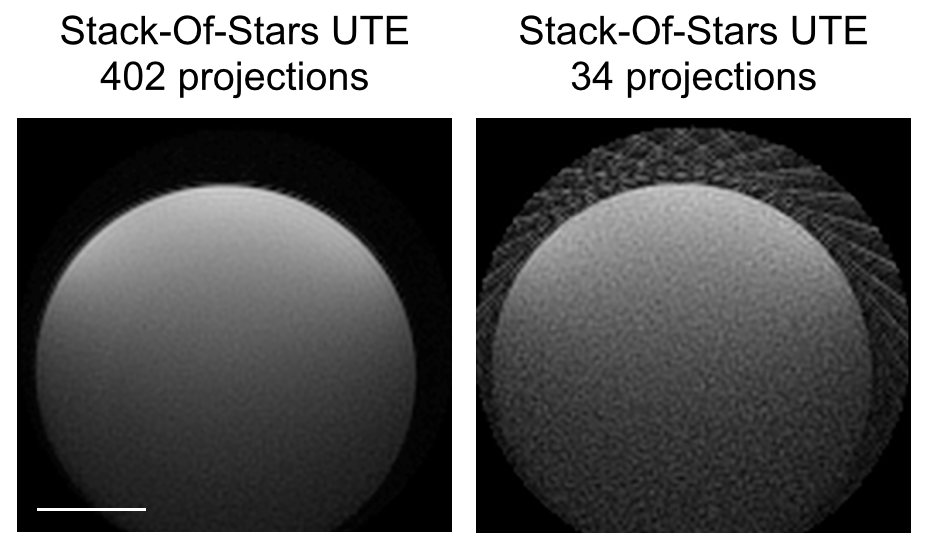
\includegraphics[scale=0.5]{./figure/chap5/Fig1.png}
\caption[Effet du sous-échantillonnage avec une séquence 3D-SOS UTE.]{\label{fig:SoSUTE} \textbf{Effet du sous-échantillonnage avec une séquence 3D-SOS UTE.} Images obtenues sur un fantôme d'eau avec une séquence Stack-Of-Stars UTE avec 402 projections par plan à gauche et 34 projections par plan à droite. On observe des artefacts de "streaking" particulièrement visibles en dehors du fantôme. La barre d'échelle représente 7,5 mm.}
\line(1,0){400} \\ 
\end{figure}

La séquence a été modifiée pour permettre de recueillir un signal d'écho-navigateur et est présentée dans la figure \ref{fig:SeqSoSUTE}. Généralement, les gradients de rephasage de coupe et de codage de phase dans la direction de coupe sont appliqués en même temps. Ici, les deux gradients sont séparés pour permettre de recueillir le signal d'écho-navigateur au centre de l'espace de Fourier entre le gradient de rephasage de coupe et la table d'encodage de coupe. 
Pour minimiser le temps d'écho, la durée des gradients a été optimisée pour obtenir des délais respectivement de 54 $\mu s$ et de 315 $\mu s$.  Le nombre de points à recueillir, indiqué en vert sur la figure \ref{fig:SeqSoSUTE}, peut être modifié pour accumuler le signal. Durant nos expériences celui-ci a été fixé à 3 correspondant à un temps d'acquisition de 30 $\mu s$ (3 x la durée d'acquisition entre deux points).

402 projections ont été recueillies par partition (Stack) dont les trajectoires sont définies selon deux méthodes : 1) méthode incrémentale $\Phi = i \times \frac{360\degres}{N_p}$, 2) la méthode d'angle d'or 2D $\Phi = i \times 222.48\degres mod(360\degres)$ où $N_p$ est le nombre de projections par partition selon la direction de coupe. Toutes les projections d'une partition sont recueillies avant le passage à la partition suivante. 96 partitions ont été recueillies durant nos expériences pour remplir un espace de Fourier cylindrique.

La méthode employée ici étant une stratégie de reconstruction rétrospective, ce schéma d'acquisition est répété un nombre de fois égal au nombre de répétitions NR. Lors de ces travaux les données ont été recueillies avec un nombre ${NR}=10$ puis sous-échantillonnée \textit{a posteriori} pour évaluer la robustesse de l'acquisition au sous-échantillonnage.

\begin{figure}[H]
\centering
\line(1,0){400} \\
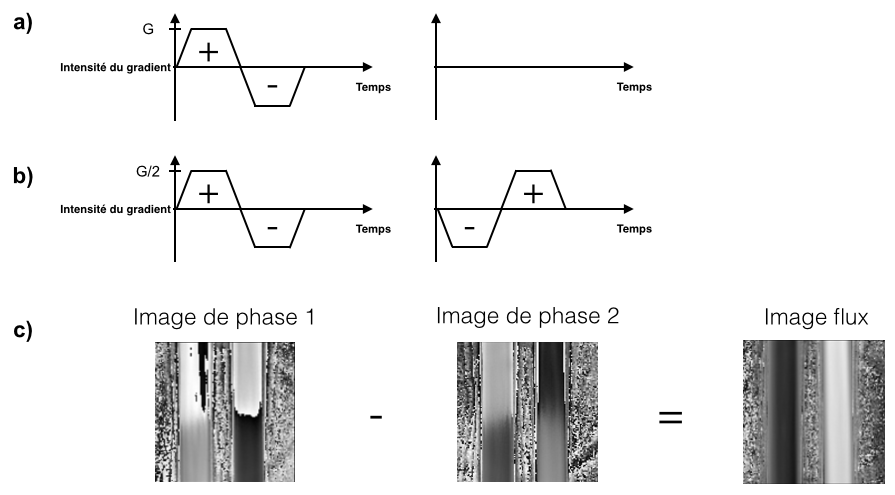
\includegraphics[scale=0.5]{./figure/chap5/Fig2.png}
\caption[Chronogramme de la séquence Stack-Of-Stars UTE auto-synchronisée sur le rythme cardiaque.]{\label{fig:SeqSoSUTE}\textbf{Chronogramme de la séquence Stack-Of-Stars UTE auto-synchronisée sur le rythme cardiaque.} Le signal d'écho-navigateur (en vert) est recueilli durant le gradient de rephasage de coupe. Le signal utilisé pour la reconstruction est indiqué en rouge et est encodé selon une trajectoire incrémentale ou d'angle d'or 2D.}
\line(1,0){400} \\ 
\end{figure}

\subsection{Traitement du signal d'écho-navigateur.}

Le signal d'écho-navigateur est utilisé pour extraire les mouvements de contraction du coeur \textit{a posteriori} en utilisant le logiciel MATLAB (MathWorks, Natick, MA).  Les points recueillis sont additionnés de manière complexe pour chaque élément d'antenne. L'élément permettant d'obtenir la plus grande amplitude de variation de signal est utilisé et son signal est convolué avec un filtre gaussien pour limiter les effets du bruit sur la détection des pics (voir figure \ref{fig:Signal}). Le début de chaque cycle cardiaque est déterminé grâce à un algorithme de détection des pics.  L'écart médian entre les pics ainsi que son écart-type sont calculés. Les données recueillies entre deux pics qui sont distants de plus de 2 fois l'écart-type par rapport à la valeur médiane ne sont pas utilisées durant la reconstruction.

Le nombre de volumes ciné (NCiné) reconstruits durant le mouvement cardiaque est défini par l'utilisateur. Les données sont regroupées en fonction de leur position relative entre deux pics de l'écho-navigateur dans les espaces de Fourier correspondant au cycle cardiaque permettant ensuite de reconstruire les volumes cinés avec la procédure de reconstruction "gridding" évoquée dans le chapitre \ref{Chap2}.

\begin{figure}[H]
\centering
\line(1,0){400} \\
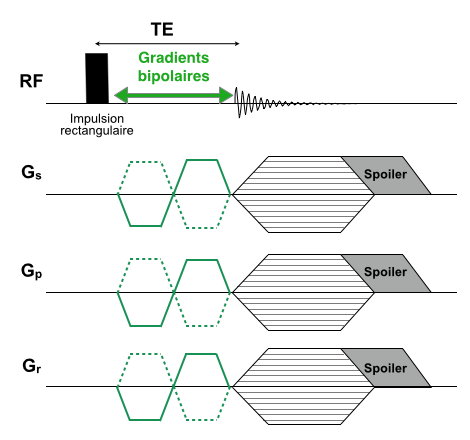
\includegraphics[scale=0.35]{./figure/chap5/Fig3.png}
\caption[Extraction du signal d'écho-navigateur.]{\label{fig:Signal} \textbf{Extraction du signal d'écho-navigateur.} Schéma présentant le signal écho-navigateur cardiaque obtenu durant une acquisition sur une souris avec une séquence \textbf{(a)} UTE 2D sans injection et \textbf{(b)}Stack-Of-Stars UTE 3D avant injection et \textbf{(c)} après injection de 200 $\mu mol Fe/kg$ de Sinerem. Le signal brut est présenté sur le schéma du haut et après convolution avec un filtre gaussien sur le schéma du bas. Les images axiales du coeur correspondantes sont présentées en bas. La barre d'échelle représente 5 mm.}
\line(1,0){400} \\ 
\end{figure}

Des exemples de signaux d'écho-navigateur sont montrés dans la figure \ref{fig:Signal} pour une acquisition 2D et 3D sans injection de produit de contraste et après injection de 200 $\mu mol Fe/kg$. 

Le signal d'écho-navigateur obtenu avec la version 2D de la séquence, sans injection d'agent de contraste, et une épaisseur de coupe de 0,3 mm est montré dans la figure \ref{fig:Signal}.a. Comme décrit dans la littérature, le cycle cardiaque et respiratoire peut être extrait des données brutes avec ou sans filtrage et des images peuvent être reconstruites rétrospectivement. Quand l'épaisseur de coupe est augmentée pour réaliser l'imagerie 3D (figure \ref{fig:Signal}.b), l'amplitude des pics provoquée par le mouvement respiratoire semble comparable à celle de l'image 2D. D'un autre côté, l'amplitude de variation de signal provoquée par le mouvement cardiaque est diminuée et le niveau de bruit est fortement augmenté. Dans certain cas, le signal peut être filtré et permet d'obtenir une visualisation suffisament précise des pics pour permettre d'assigner les projections dans les cycles cardiaques correspondants comme montré sur la figure \ref{fig:Signal}.b. Cependant, dans certaines expériences le niveau de bruit est trop important et empêche une détection précise des pics et donc une reconstruction rétrospective. Une fois de plus, le problème majeur avec les acquisitions 3D est l'absence de signal sanguin dans le ventricule gauche ($\text{SSB}= 9,57 \pm 2,19$ et $\text{CSB}= -7,82 \pm 2,05$) provoquée par la saturation du signal du sang. Cette absence de contraste empêche d'effectuer des analyses de volumétrie cardiaque.
Après l'injection d'un agent de contraste à base de nanoparticules de fer, le signal sanguin dans les deux ventricules est rehaussé ($\text{SSB}= 42,25 \pm 2,19$ et $\text{CSB}= 17,25 \pm 2,34$) comme montré dans la figure \ref{fig:Signal}.c. La variation d'amplitude provoquée par le mouvement cardiaque est alors augmentée et le bruit est faible par rapport au signal sans agent de contraste. Des images ciné peuvent être reconstruites après que les projections aient été assignées au cycle cardiaque correspondant. Ces images peuvent être utilisées pour effectuer des analyses de la fonction cardiaque. Entre 5 et 10  pourcents du nombre total de projections acquises durant l'expérience sont généralement rejetées en raison d'une trop grande déviation par rapport au rythme médian. Le rythme cardiaque moyen mesuré dans les expériences a été de $412 \pm 32$ et $370 \pm 53$ bpm respectivement pour les souris saines et pour les souris ischémiques.

\section{Répartition des projections selon la méthode de l'angle incrémental ou selon la méthode de l'angle d'or 2D.}

Dans le cas d'une reconstruction rétrospective la méthode de répartition des projections au cours du temps a une influence sur le résultat. Par exemple dans le cas de la suppresion des projections corrompues par la respiration, avec une trajectoire incrémentale une partie de l'espace de Fourier n'est pas remplie car les projections sont adjacentes alors qu'avec une trajectoire aléatoire, ces suppressions de projection sont réparties dans tout l'espace de Fourier et non pas centralisées autour d'une position. 

Pour valider cette affirmation dans le cas d'une séquence cardiaque 3D avec une trajectoire basée sur l'angle d'or 2D, une analyse de la densité de l'espace de Fourier a été effectuée en fonction des méthodes d'encodage (méthode incrémentale versus angle d'or 2D). Deux paramètres ont été étudiés : l'angle moyen et l'écart-type entre les projections les plus proches dans chaque partition. Cette analyse a été effectuée sur des données acquises \textit{in vivo} sur 4 souris saines pour obtenir 10 images ciné, rétrospectivement sous-échantillonnées (de $NR = 10$ à $NR = 1$).

La figure \ref{fig:GoldVSIncNr}.a montre la valeur moyenne de l'angle en fonction du nombre de répétitions. Les deux méthodes permettent d'obtenir des résultats quasi-identiques avec des valeurs inférieures à 2$\degres$ pour un nombre de répétitions supérieur à 7 puis qui augmentent jusqu'à 9$\degres$ pour une seule répétition. En revanche, en ce qui concerne l'écart-type de la valeur de l'angle, la méthode avec l'angle d'or 2D permet d'obtenir des valeurs toujours plus faibles par rapport à la méthode utilisant l'angle incrémental.% Il est à noté que la dispersion de ces écart-types augmente avec la diminution du nombre de répétition. Cela peut s'expliquer par la différence de rythme cardiaque ainsi que d'efficacité de détection des pics entre les animaux.

\begin{figure}[H]
\centering
\line(1,0){400} \\
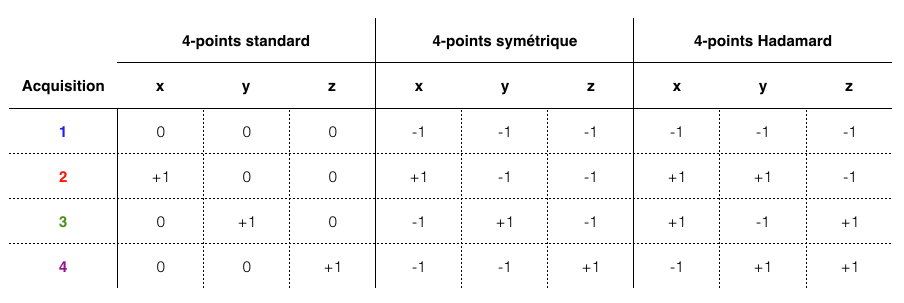
\includegraphics[scale=0.6]{./figure/chap5/Fig4.png}
\caption[Mesure de la densité de répartition des projections.]{\label{fig:GoldVSIncNr} \textbf{Mesure de la densité de répartition des projections.} Graphiques représentant \textbf{(a)} la moyenne et \textbf{(b)} l'écart-type des angles entre les projections les plus proches dans une même partition, en fonction du nombre de NR utilisés pour la reconstruction. Les paramètres sont affichés pour la répartition incrémentale des projections et selon l'angle d'or 2D.}
\line(1,0){400} \\ 
\end{figure}

Des images réprésentatives reconstruites en vue long et petit axes sont montrées sur la figure \ref{fig:ImGoldVSIncNr} obtenues avec les deux méthodes de répartition des projections sur une souris saine et avec un nombre de répétitions décroissant.

\begin{figure}[H]
\centering
\line(1,0){400} \\
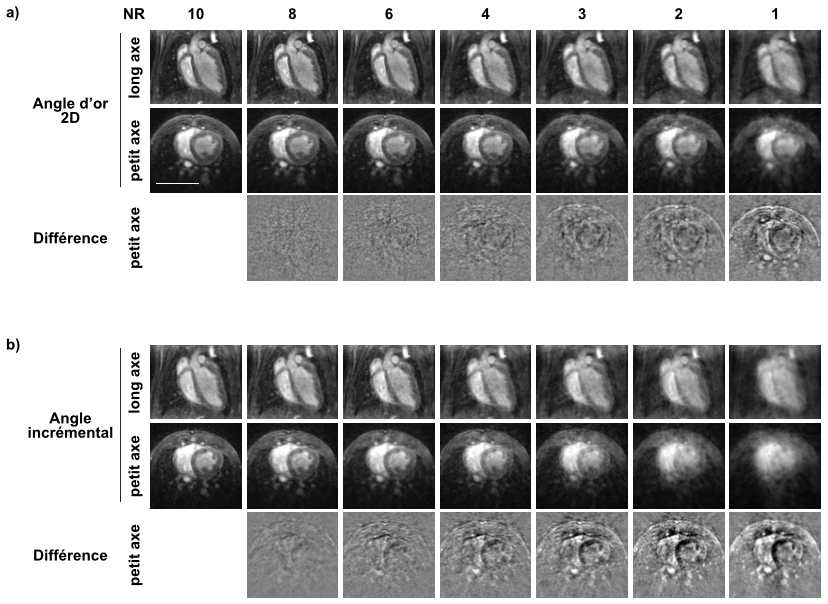
\includegraphics[scale=0.5]{./figure/chap5/Fig5.png}
\caption[Influence de la trajectoire sur la qualité des images.]{\label{fig:ImGoldVSIncNr} \textbf{Influence de la trajectoire sur la qualité des images en fonction du sous-échantillonnage.} Images long et petit axes d'un coeur de souris saine reconstruites avec un nombre décroissant de répétitions (NR) avec : \textbf{a)} une répartition selon l'angle d'or 2D \textbf{b)} une répartition selon l'angle incrémental. Une image de différence est aussi présentée sur la dernière ligne. La barre d'échelle représente 10 mm.}
\line(1,0){400} \\ 
\end{figure}

Avec le nombre maximum de répétitions (NR = 10), les images obtenues sont de qualités comparables. Le sang à l'intérieur du coeur apparaît avec un signal parfaitement homogène et sans artefact de flux. Le rapport contraste-sur-bruit entre le sang et le myocarde est d'environ 15 avec les deux méthodes (figure \ref{fig:TabGoldVSIncNr}). En diminuant le nombre de répétitions, la qualité des images décroît plus rapidement avec la méthode incrémentale. Ceci est également visible sur les images de différences obtenues par soustraction de l'image avec NR = 10 avec les images obtenues avec des NR plus faibles.
La résolution spatiale des images est dégradée et le contraste-sur-bruit entre le sang et le myocarde diminue plus fortement sur les images obtenues avec l’angle incrémental (figure \ref{fig:TabGoldVSIncNr}). En diminuant nettement le nombre de répétitions (NR = 2 et 1), la visualisation des ventricules et des parois du myocarde reste possible avec la méthode d'angle d’or 2D mais impossible avec l’autre méthode.

\begin{figure}[H]
\centering
\line(1,0){400} \\
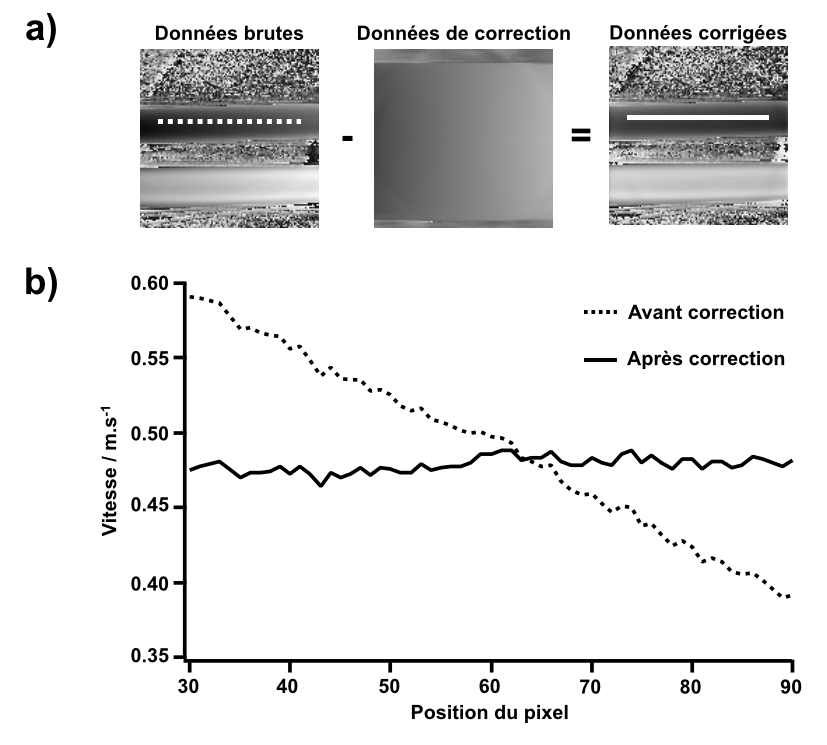
\includegraphics[scale=0.6]{./figure/chap5/Fig6.png}
\caption[Tableau des valeurs de CSB entre les méthodes de répartition d'angle d'or 2D et incrémentale.]{\label{fig:TabGoldVSIncNr} \textbf{Tableau des valeurs de CSB entre les méthodes de répartition d'angle d'or 2D et incrémentale.} Les mesures de CSB ont été effectuées entre le sang et le myocarde pour différentes valeurs de sous-échantillonnage (NR = 10 à 1).}
\line(1,0){400} \\ 
\end{figure}


La flexibilité de cette méthode d'auto-synchronisation permet d'augmenter le nombre d'images ciné reconstruites à partir d'un même jeu de données. L'écart-type de l'angle entre les projections pour chaque méthode de répartition des projections est représenté dans la figure \ref{fig:GoldVSIncNCine} en fonction du nombre d'images ciné reconstruites. Les données utilisées dans chaque graphique correspondent à cette mesure effectuée sur des données avec un nombre de répétitions décroissant (NR égale à 10, 8, 6 et 4). La méthode d'angle d'or 2D reste plus efficace et l'écart de la valeur reste stable entre les deux méthodes jusqu'à un nombre d'images ciné égal à 20. Après cette valeur, les deux techniques présentent des valeurs qui se rapprochent.

\begin{figure}[H]
\centering
\line(1,0){400} \\
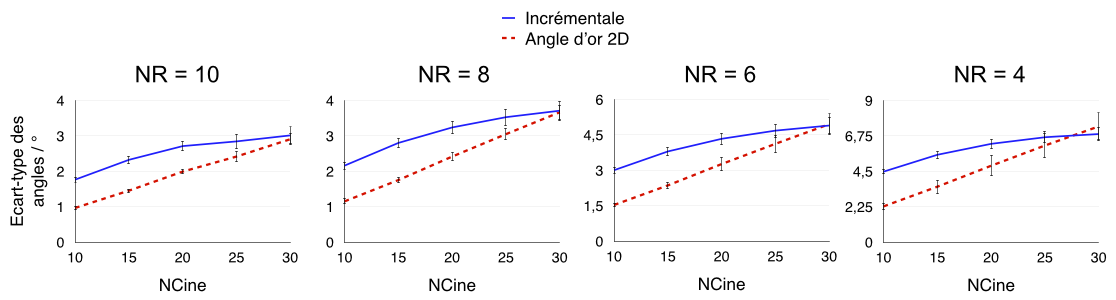
\includegraphics[scale=0.4]{./figure/chap5/Fig7.png}
\caption[Quantification de l'écart-type des angles en fonction de nombre d'images ciné reconstruitent.]{\label{fig:GoldVSIncNCine} \textbf{Quantification de l'écart-type des angles en fonction de nombre d'images ciné reconstruitent.} Graphique représentant  l'écart-type des angles entre les projections les plus proches dans une même partition en fonction du nombre de volumes ciné reconstruits pour la répartition incrémentale et selon l'angle d'or 2D. Les mesures sont représentées en fonction du nombre de répétitions (NR) utilisé pour la reconstruction.}
\line(1,0){400} \\ 
\end{figure}

\section{Imagerie d'un modèle sain de souris par rapport à un modèle d'infarctus du myocarde aiguë}

L'imagerie des souris a été effectuée à 7 Tesla avec une antenne surfacique à 4 éléments. Les paramètres d'acquisitions sont les suivants :
TR/TE = 4/0.552 ms, type d'excitation radiofréquence/durée/angle d'excitation = hermite/0,3 ms/15$\degres$, champ de vue = 20 x 20 x 15 mm, matrice dans le plan = 128 x 128, nombre de partitions = 96, nombre de projections par partition = 402, bande passante de réception = 781 Hz/Pixel, nombre de répétitions = 10, temps d'acquisition total : 25 min 43 sec, 3 points recueillis pour l'écho-navigateur.

Des souris OF1 saines (n=4) et avec un infarctus du myocarde (n=4) avec un poids compris entre 37 et 40g ont été imagées. Les souris ont été injectées avec un volume de 150 $\mu L$ de Sinerem (Guerbet, Aulnay-sous-bois, France) à une concentration de 200 $\mu mol$ Fe/kg avant le positionnement dans l'imageur.

\newpage
\subsection{Qualité des images}

La figure \ref{fig:ImSaine} montre les 10 images ciné en orientation long et petit axes obtenues chez une souris saine avec un nombre de répétitions égale à 6. La figure \ref{fig:ImInfarct} montre les images obtenues sur une souris avec une ischémie sévère du myocarde. La vue long axe est montrée sur la première ligne (\ref{fig:ImInfarct}.a) et des coupes aux positions b, c et d (indiquées sur la figure \ref{fig:ImInfarct}.a.1) sont montrées sur les autres lignes.

Sur les deux types de souris, le sang apparaît avec un signal intense et homogène sans artefact de flux, quel que soit le moment du cycle cardiaque. Grâce à l'acquisition 3D, l'entièreté de la zone ischémiée chez les souris pathologiques peut être délimitée sur les différentes orientations des images (voir flèches sur la figure \ref{fig:ImInfarct}).

\begin{figure}[H]
\centering
\line(1,0){400} \\
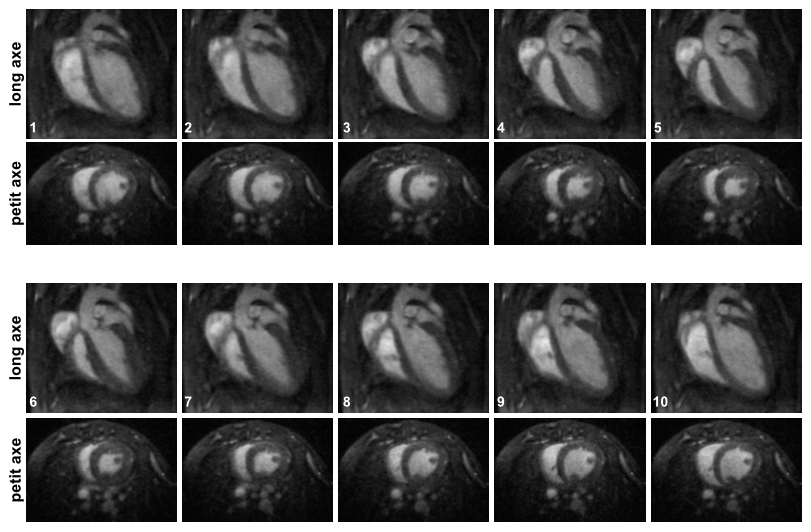
\includegraphics[scale=0.5]{./figure/chap5/Fig8.png}
\caption[Images 3D obtenues sur une souris saine avec la séquence 3D-SOS UTE auto-synchronisée.]{\label{fig:ImSaine} \textbf{Images 3D obtenues sur une souris saine avec la séquence 3D-SOS UTE auto-synchronisée.} 10 images ciné 3D (orientation long axe et orientation petit axe) obtenues chez une souris saine avec la séquence 3D-SOS UTE auto-synchronisée, la répartition des projections par la méthode de l’angle d’or 2D et un nombre de répétitions NR = 6.}
\line(1,0){400} \\ 
\end{figure}

\begin{figure}[H]
\centering
\line(1,0){400} \\
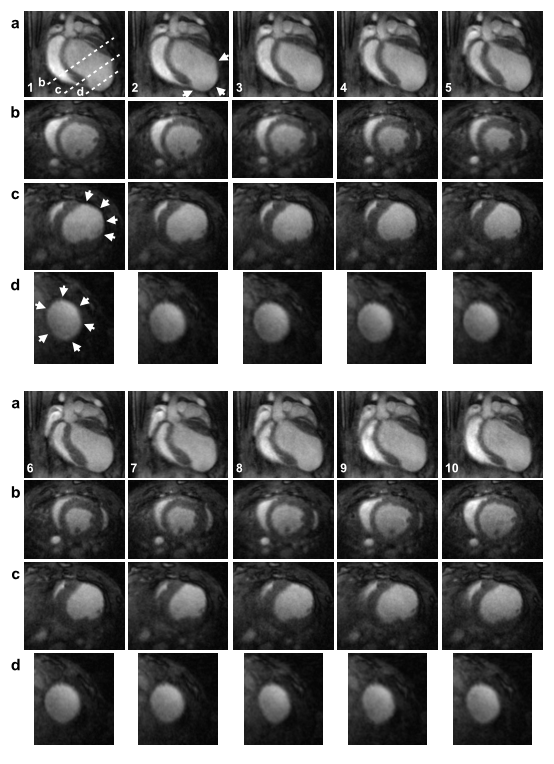
\includegraphics[scale=0.6]{./figure/chap5/Fig9.png}
\caption[Images 3D obtenues sur une souris avec un infarctus du myocarde avec la séquence 3D-SOS UTE auto-synchronisée.]{\label{fig:ImInfarct} \textbf{Images 3D-t obtenues sur une souris avec un infarctus du myocarde avec la séquence 3D-SOS UTE auto-synchronisée.} 10 images ciné 3D obtenues chez une souris avec un infarctus du myocarde avec la séquence 3D-SOS UTE auto-synchronisée; la répartition des projections par la méthode de l’angle d’or et un nombre de répétitions NR = 6. Ligne a) orientation long axe. La position des coupes montrées en b) c) et d) apparaît sur l’image 1.a). Les flèches indiquent la zone ischémique.}
\line(1,0){400} \\ 
\end{figure}


\subsection{Quantification de la fonction cardiaque.}

Les volumes du ventricule gauche en fin de diastole et de systole ont été mesurés puis la fraction d'éjection calculée à partir des images acquises sur les souris saines et pathologiques. Les valeurs moyennes de la fraction d'éjection, du volume de fin de diastole et de fin de systole du ventricule gauche apparaissent fortement différentes entre les deux types de souris pour la valeur NR = 10 (voir figure \ref{fig:TabFractionEjection})

\begin{figure}[H]
\centering
\line(1,0){400} \\
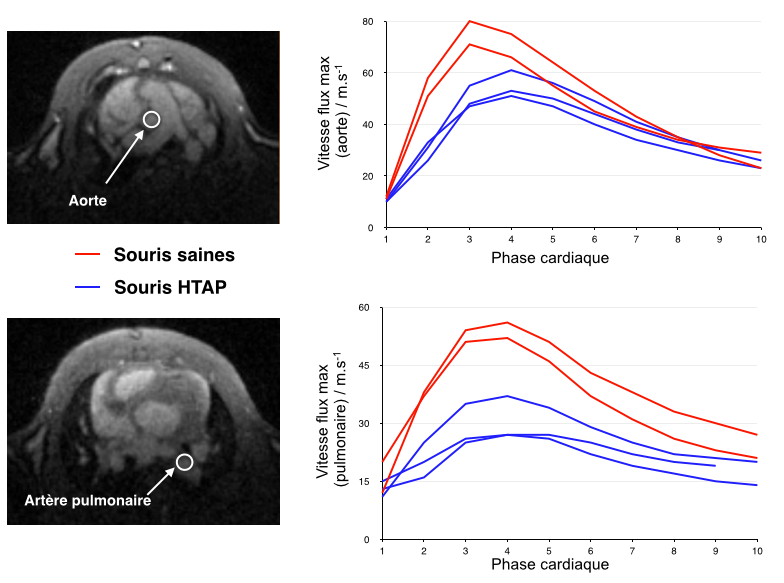
\includegraphics[scale=0.5]{./figure/chap5/Fig10.png}
\caption[Tableau des volumes et fractions d'éjection pour les souris saines et pathologiques.]{\label{fig:TabFractionEjection} \textbf{Tableau des volumes et fractions d'éjection pour les souris saines et pathologiques.} Valeurs moyennes de la fraction d’éjection (FE), du volume de fin de diastole (VD) et du volume de fin de systole (VS) obtenues chez les souris saines et les souris avec un infarctus du myocarde.}
\line(1,0){400} \\ 
\end{figure}

Les mesures ont aussi été réalisées sur les images reconstruites avec NR = 6 et 3. Les données avec NR = 10 ont été prises comme référence. Les données obtenues avec NR = 6 sont extrêmement proches des données obtenues avec NR : 10 pour les deux types de souris. En revanche, avec NR = 3 les données obtenues sur souris saines apparaissent plus dispersées comme le montre le graphique de Bland-Altman sur la figure \ref{fig:BlandAltmanFractionEjection}.

\begin{figure}[H]
\centering
\line(1,0){400} \\
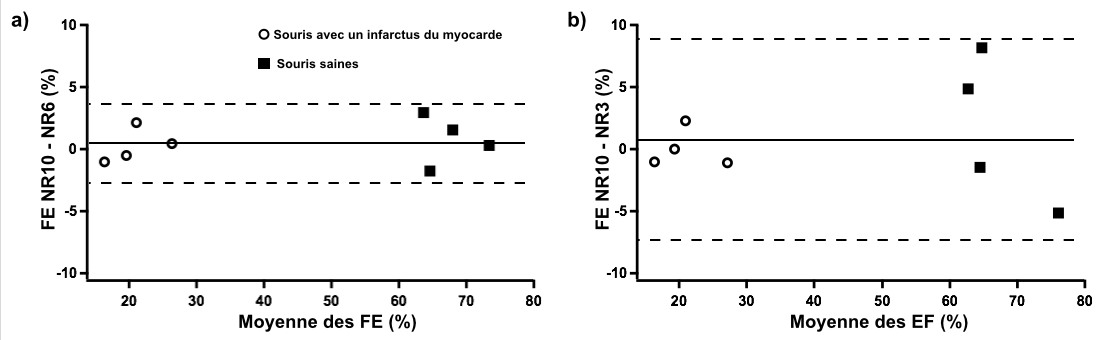
\includegraphics[scale=0.4]{./figure/chap5/Fig11.png}
\caption[Graphique de Bland-Altman de la fraction d’éjection.]{\label{fig:BlandAltmanFractionEjection} \textbf{Graphique de Bland-Altman de la fraction d’éjection.} \textbf{a)} NR = 6 et \textbf{b)} NR = 3 en comparaison à NR = 10. Les carrés pleins indiquent les souris saines et les ronds vides les souris avec infarctus du myocarde.}
\line(1,0){400} \\ 
\end{figure}

\subsection{Quantification de la fonction cardiaque en fonction de la zone du coeur.}

Grâce au caractère 3D des données et aux résolutions isotropes obtenues, les analyses volumiques et de fractions d'éjection peuvent être réalisées coupe à coupe du haut jusqu'au bas du coeur.
Pour la souris saine montrée sur la figure \ref{fig:FractionEjectionCoupe}.a le coeur est ainsi divisé en 40 coupes. La fraction d'éjection apparaît quasi constante tout le long du grand axe et avec des valeurs aux alentours de la fraction d'éjection moyenne. Des profils identiques ont été observés sur les autres souris saines.

Pour la souris avec un infarctus du myocarde montrée sur la figure \ref{fig:FractionEjectionCoupe}.b, le coeur est divisé en 55 coupes. La valeur de fraction d'éjection dans le haut du coeur est comparable à la souris saine environ jusqu'à la coupe 15. Elle diminue ensuite fortement pour être nulle à partir de la coupe 40.

\begin{figure}[H]
\centering
\line(1,0){400} \\
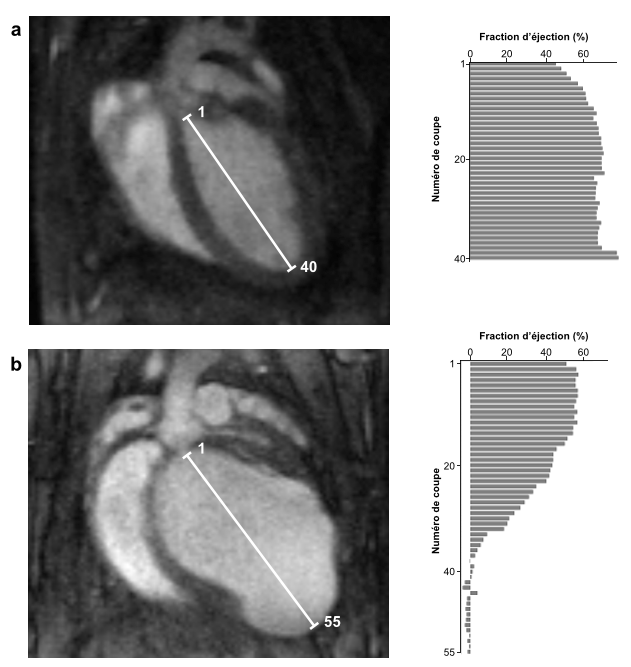
\includegraphics[scale=0.5]{./figure/chap5/Fig12.png}
\caption[Analyse de la fraction d'éjection en fonction de la position dans le coeur.]{\label{fig:FractionEjectionCoupe} \textbf{Analyse de la fraction d'éjection en fonction de la position dans le coeur.} Les données présentées correspondent à une souris saine (a) et à une souris avec un infarctus du myocarde (b). Le segment representé sur les images est perpendiculaire à la position des coupes.}
\line(1,0){400} \\ 
\end{figure}

\section{Discussion}


Une méthode d’imagerie 4D pour la mesure de la fonction du ventricule gauche chez la souris a été développée et utilisée pour la caractérisation de souris saines et de souris atteintes d’un infarctus sévère du myocarde.
La méthode se base sur un encodage hybride, radial à temps d’écho ultracourts dans la dimension du plan et cartésien dans la dimension de coupe. 

L’utilisation de l’encodage cartésien dans la 3ème dimension a plusieurs avantages. Le premier est qu’il permet de réaliser une sélection de coupe relativement fine et ainsi obtenir un signal d’auto-synchronisation cardiaque \cite{crowe2004automated}. En effet, avec une méthode UTE purement radiale (3D-UTE) le signal d’auto-synchronisation cardiaque est noyé dans le signal d’un large volume, même après injection d’USPIO (données non montrées) et il n’apparaît pas assez intense pour extraire le rythme cardiaque de l’animal. Avec la séquence proposée, le signal d’écho-navigateur est lu pendant le gradient de refocalisation de coupe. Contrairement aux séquences UTE 2D classiques, le premier point du signal UTE \cite{Hoerr:2013gf,Motaal:2015aa}, échantillonné au centre de l’espace-k ne peut être utilisé comme écho-navigateur. Il est en plus nécessaire d’ajouter une table de codage dans la direction de coupe. Le temps d’écho est ainsi rallongé en 3D. Toutefois, en compressant la séquence et en utilisant des gradients de codage intenses, il a été possible de limiter le temps d’écho à environ 0.5 ms. Avec cette méthode, comme déjà proposé avec les séquences 2D, le signal d’écho-navigateur est lu à chaque TR contrairement à certaines études chez l’homme \cite{coppo2014free} et le petit animal \cite{kramer2015self} où le signal de l’écho-navigateur n’est lu que périodiquement (tout les 4 ou 10 TR). Cela permet, chez la souris où le rythme cardiaque est extrêmement élevé, d’identifier avec précision le signal de synchronisation cardiaque. 
\medskip

L’autre avantage de cette séquence utilisant un encodage cartésien dans la direction de coupe est la possibilité de limiter le champ de vue dans la troisième direction et ainsi le temps d’acquisition. Néanmoins, malgré une coupe limitée en épaisseur, le sang dans les cavités cardiaque apparaît saturé. Il n’est pas possible de visualiser le sang dans le ventricule gauche de l’animal contrairement aux acquisitions en 2D qui avec des coupes environ 10 fois plus fines bénéficient d'un effet temps-de-vol. Comme dans plusieurs autres études réalisées en 3D chez le petit animal, il a donc été nécessaire de rehausser le signal du sang avec un agent de contraste \cite{Bucholz:2008uq,Bucholz:2010aa}. 

Comme déjà montré précédemment, un agent de contraste à base de fer a été utilisé \cite{trotier2015positive}. En effet, ces agents présentent l’avantage d’avoir une forte rémanence vasculaire et de générer un contraste positif avec les séquences UTE, même à hauts champs magnétiques \cite{Gharagouzloo2015Quantitative-co}. Du fait de l’autorisation FDA du Ferumoxytol comme supplément en fer pour les patients victimes d’anémies chroniques, ces agents connaissent un regain d’intérêt pour l’angiographie chez l’homme et l’animal \cite{ruangwattanapaisarn2014ferumoxytol}. L’augmentation du temps d’écho (TE = 0.552 ms) d’un facteur 15 environ par rapport aux travaux publiés récemment (TE = 0.031 ms), a peu d’influence sur le signal généré avec les concentrations utilisées dans cet article. Le sang conserve un signal intense tout au long de l’expérience. En effet, grâce à l’encodage SOS-UTE 3D, le temps d’écho de la séquence reste bien en dessous de la milliseconde. De plus, ce type d’encodage rend la séquence peu sensible aux artefacts de mouvements et aux artefacts de flux (même dans sa version 3D). Une synchronisation respiratoire n’a donc pas besoin d’être mise en place. Ainsi, le signal du sang apparaît homogène tout au long du cycle cardiaque et chez les deux modèles de souris. Ceci permet de réaliser une segmentation sans ambiguité et d'obtenir une mesure précise du volume des ventricules. 

Les séquences à TE ultracourts sont également favorables au sous-échantillonnage. Il n’est donc pas nécessaire de générer un espace de Fourier complet pour obtenir une image. Ainsi dans le cas d'une reconstruction retrospective, la combinaison de cet encodage permet de générer des images de bonne qualité sans répondre au critère de Nyquist. Cependant, avec une trajectoire classique de type incrémental, la répartition des projections obtenues n’est pas parfaitement homogène, en particulier avec un nombre de répétitions faibles. Cela se traduit par l’apparition d'artefacts typiques de l'encodage radial (artefact de « streaking »).
Afin d’améliorer cette situation, une trajectoire pseudo-aléatoire basée sur l’angle d’or (ou golden angle) de chaque disque a été implantée. Comme montré ici, l’utilisation de celle-ci en combinaison avec la méthode de reconstruction rétrospective permet d’obtenir une répartition plus homogène des projections à l’intérieur d’une partition. Ainsi, des images 3D fortement sous échantillonnées peuvent être obtenues avec une meilleure résolution spatiale. Ceci peut être utilisé pour limiter le temps d’acquisition des images, pour compenser des données perdues par un mauvais signal de l’écho-navigateur ou enfin pour reconstruire un nombre plus important d’images ciné par cycle cardiaque. Ici, seul un encodage aléatoire a été utilisé à l’intérieur de chaque empilement. Du fait du caractère 3D de la séquence, il pourrait être envisagé d’étendre ce caractère pseudo-aléatoire entre les différents empilements pour encore plus limiter les artefacts de reconstruction.

En combinant les différents avantages de la séquence développée, nous avons montré qu’il était possible d’obtenir des images 3D ciné sans synchronisation ECG chez la souris saine et la souris avec un infarctus du myocarde sévère. Le signal d’auto-synchronisation, après injection de nanoparticules de fer, s’est montré de qualité suffisante, même chez les souris avec un infarctus. Des résolutions élevées ont été atteintes dans les 3 dimensions de l’espace et permettent ainsi de décrire les modèles pathologiques beaucoup plus finement que ce qui était jusqu’à aujourd’hui décrit dans la littérature. En effet, en imagerie 2D l’épaisseur de coupe est en général limitée à 0,8 mm \cite{Bovens:2011aa,Hoerr:2013gf}, le nombre de coupe utilisé sur le coeur entier est au maximum de 10. Ici, 40 pseudo-coupes reconstruites peuvent être utilisées pour déterminer les paramètres fonctionnels cardiaques chez les souris saines et 55 chez les souris avec un infarctus du myocarde. Grâce à ces données, la pathologie peut être décrite en détail dans les 3 dimensions du coeur. La méthode utilisée permet également de limiter le temps d’acquisition des séquences, paramètre primordiale lors d’études chez des animaux fragiles. Le nombre de répétitions fixé initialement à 10 (temps d’acquisition = 25 min 43 sec) peut ainsi être limité avec très peu de perte en qualité d’image et ainsi obtenir un temps d’acquisition de 15 min 26 sec pour NR = 6. La mesure des paramètres fonctionnels reste extrêmement robuste. En diminuant ce nombre de répétitions à 3 (temps d’acquisition = 7 min 52 sec) l’erreur devient plus importante mais reste acceptable. 

En résumé, dans ce travail nous présentons une méthode, rehaussée par des nanoparticules de fer, pour l’imagerie ciné 3D du coeur de souris avec une séquence hybride radiale-cartésienne à TE ultracourt. La technique utilise une méthode d’auto-synchronisation couplée à un encodage pseudo-aléatoire des données et permet de mesurer les paramètres fonctionnels cardiaques chez des souris saines et avec un infarctus du myocarde avec des résolution spatiales encore inégalées et un temps d’acquisition de l’ordre de 15 minutes. 


\section{Limitation}

La position du coeur par rapport aux canaux de l'antenne influence le signal d'écho-navigateur, il est donc nécessaire de sélectionner le canal optimal permettant la visualisation et l'extraction des pics. 

 Il peut également arriver que le signal d'écho-navigateur soit trop faible et nécessite donc une modification de la position de l'animal ou des paramètres d'acquisitions, par exemple une réduction de champ de vue selon la direction de coupe centrée sur le coeur.

\section{Perspectives}
\begin{enumerate}

\item La principale amélioration à apporter à ce travail se situe au niveau du traitement du signal d'écho-navigateur pour permettre une extraction totalement automatique des pics cardiaques, c'est-à-dire sans intervention d'un opérateur. Plusieurs stratégies sont à explorer comme la convolution avec un autre type de filtre dont les paramètres seront adaptés aux variations du signal spécifiques des données chez le petit animal. Une autre alternative serait d'utiliser une corrélation croisée entre les signaux des différents canaux de l'antenne.

\item Cette méthode est particulièrement adaptée à l'utilisation de stratégies permettant d'améliorer la résolution spatiotemporelle comme les filtres temporels présentés dans le chapitre \ref{Chap3} ou bien avec des méthodes d'accélération de type kt-space puisque l'aspect rétrospectif permet de remplir de manière "aléatoire" les espaces au cours du temps \cite{Motaal:2015aa}.

\item L'ajout de la troisième dimension permet de multiplier les possibilités de quantification. Cependant des outils de traitement et d'analyse de données restent à développer pour permettre des études de plus grandes cohortes par exemple dans le cas d'études visant à quantifier la réponse à des traitements pharmacologiques ou à des méthodes de reperfusion du coeur dans le cas d'infarctus ou d'ischémie.
\end{enumerate}



